\documentclass[]{book}
\usepackage{lmodern}
\usepackage{amssymb,amsmath}
\usepackage{ifxetex,ifluatex}
\usepackage{fixltx2e} % provides \textsubscript
\ifnum 0\ifxetex 1\fi\ifluatex 1\fi=0 % if pdftex
  \usepackage[T1]{fontenc}
  \usepackage[utf8]{inputenc}
\else % if luatex or xelatex
  \ifxetex
    \usepackage{mathspec}
  \else
    \usepackage{fontspec}
  \fi
  \defaultfontfeatures{Ligatures=TeX,Scale=MatchLowercase}
\fi
% use upquote if available, for straight quotes in verbatim environments
\IfFileExists{upquote.sty}{\usepackage{upquote}}{}
% use microtype if available
\IfFileExists{microtype.sty}{%
\usepackage{microtype}
\UseMicrotypeSet[protrusion]{basicmath} % disable protrusion for tt fonts
}{}
\usepackage[margin=1in]{geometry}
\usepackage{hyperref}
\hypersetup{unicode=true,
            pdftitle={R for FinTech},
            pdfauthor={Jasmine Dumas},
            pdfborder={0 0 0},
            breaklinks=true}
\urlstyle{same}  % don't use monospace font for urls
\usepackage{natbib}
\bibliographystyle{apalike}
\usepackage{color}
\usepackage{fancyvrb}
\newcommand{\VerbBar}{|}
\newcommand{\VERB}{\Verb[commandchars=\\\{\}]}
\DefineVerbatimEnvironment{Highlighting}{Verbatim}{commandchars=\\\{\}}
% Add ',fontsize=\small' for more characters per line
\usepackage{framed}
\definecolor{shadecolor}{RGB}{248,248,248}
\newenvironment{Shaded}{\begin{snugshade}}{\end{snugshade}}
\newcommand{\KeywordTok}[1]{\textcolor[rgb]{0.13,0.29,0.53}{\textbf{{#1}}}}
\newcommand{\DataTypeTok}[1]{\textcolor[rgb]{0.13,0.29,0.53}{{#1}}}
\newcommand{\DecValTok}[1]{\textcolor[rgb]{0.00,0.00,0.81}{{#1}}}
\newcommand{\BaseNTok}[1]{\textcolor[rgb]{0.00,0.00,0.81}{{#1}}}
\newcommand{\FloatTok}[1]{\textcolor[rgb]{0.00,0.00,0.81}{{#1}}}
\newcommand{\ConstantTok}[1]{\textcolor[rgb]{0.00,0.00,0.00}{{#1}}}
\newcommand{\CharTok}[1]{\textcolor[rgb]{0.31,0.60,0.02}{{#1}}}
\newcommand{\SpecialCharTok}[1]{\textcolor[rgb]{0.00,0.00,0.00}{{#1}}}
\newcommand{\StringTok}[1]{\textcolor[rgb]{0.31,0.60,0.02}{{#1}}}
\newcommand{\VerbatimStringTok}[1]{\textcolor[rgb]{0.31,0.60,0.02}{{#1}}}
\newcommand{\SpecialStringTok}[1]{\textcolor[rgb]{0.31,0.60,0.02}{{#1}}}
\newcommand{\ImportTok}[1]{{#1}}
\newcommand{\CommentTok}[1]{\textcolor[rgb]{0.56,0.35,0.01}{\textit{{#1}}}}
\newcommand{\DocumentationTok}[1]{\textcolor[rgb]{0.56,0.35,0.01}{\textbf{\textit{{#1}}}}}
\newcommand{\AnnotationTok}[1]{\textcolor[rgb]{0.56,0.35,0.01}{\textbf{\textit{{#1}}}}}
\newcommand{\CommentVarTok}[1]{\textcolor[rgb]{0.56,0.35,0.01}{\textbf{\textit{{#1}}}}}
\newcommand{\OtherTok}[1]{\textcolor[rgb]{0.56,0.35,0.01}{{#1}}}
\newcommand{\FunctionTok}[1]{\textcolor[rgb]{0.00,0.00,0.00}{{#1}}}
\newcommand{\VariableTok}[1]{\textcolor[rgb]{0.00,0.00,0.00}{{#1}}}
\newcommand{\ControlFlowTok}[1]{\textcolor[rgb]{0.13,0.29,0.53}{\textbf{{#1}}}}
\newcommand{\OperatorTok}[1]{\textcolor[rgb]{0.81,0.36,0.00}{\textbf{{#1}}}}
\newcommand{\BuiltInTok}[1]{{#1}}
\newcommand{\ExtensionTok}[1]{{#1}}
\newcommand{\PreprocessorTok}[1]{\textcolor[rgb]{0.56,0.35,0.01}{\textit{{#1}}}}
\newcommand{\AttributeTok}[1]{\textcolor[rgb]{0.77,0.63,0.00}{{#1}}}
\newcommand{\RegionMarkerTok}[1]{{#1}}
\newcommand{\InformationTok}[1]{\textcolor[rgb]{0.56,0.35,0.01}{\textbf{\textit{{#1}}}}}
\newcommand{\WarningTok}[1]{\textcolor[rgb]{0.56,0.35,0.01}{\textbf{\textit{{#1}}}}}
\newcommand{\AlertTok}[1]{\textcolor[rgb]{0.94,0.16,0.16}{{#1}}}
\newcommand{\ErrorTok}[1]{\textcolor[rgb]{0.64,0.00,0.00}{\textbf{{#1}}}}
\newcommand{\NormalTok}[1]{{#1}}
\usepackage{longtable,booktabs}
\usepackage{graphicx,grffile}
\makeatletter
\def\maxwidth{\ifdim\Gin@nat@width>\linewidth\linewidth\else\Gin@nat@width\fi}
\def\maxheight{\ifdim\Gin@nat@height>\textheight\textheight\else\Gin@nat@height\fi}
\makeatother
% Scale images if necessary, so that they will not overflow the page
% margins by default, and it is still possible to overwrite the defaults
% using explicit options in \includegraphics[width, height, ...]{}
\setkeys{Gin}{width=\maxwidth,height=\maxheight,keepaspectratio}
\IfFileExists{parskip.sty}{%
\usepackage{parskip}
}{% else
\setlength{\parindent}{0pt}
\setlength{\parskip}{6pt plus 2pt minus 1pt}
}
\setlength{\emergencystretch}{3em}  % prevent overfull lines
\providecommand{\tightlist}{%
  \setlength{\itemsep}{0pt}\setlength{\parskip}{0pt}}
\setcounter{secnumdepth}{5}
% Redefines (sub)paragraphs to behave more like sections
\ifx\paragraph\undefined\else
\let\oldparagraph\paragraph
\renewcommand{\paragraph}[1]{\oldparagraph{#1}\mbox{}}
\fi
\ifx\subparagraph\undefined\else
\let\oldsubparagraph\subparagraph
\renewcommand{\subparagraph}[1]{\oldsubparagraph{#1}\mbox{}}
\fi

%%% Use protect on footnotes to avoid problems with footnotes in titles
\let\rmarkdownfootnote\footnote%
\def\footnote{\protect\rmarkdownfootnote}

%%% Change title format to be more compact
\usepackage{titling}

% Create subtitle command for use in maketitle
\newcommand{\subtitle}[1]{
  \posttitle{
    \begin{center}\large#1\end{center}
    }
}

\setlength{\droptitle}{-2em}
  \title{R for FinTech}
  \pretitle{\vspace{\droptitle}\centering\huge}
  \posttitle{\par}
  \author{Jasmine Dumas}
  \preauthor{\centering\large\emph}
  \postauthor{\par}
  \predate{\centering\large\emph}
  \postdate{\par}
  \date{2016-10-30}

\usepackage{booktabs}

\begin{document}
\maketitle

{
\setcounter{tocdepth}{1}
\tableofcontents
}
\chapter{Introduction}\label{introduction}

\begin{figure}[htbp]
\centering

\includegraphics{cover.png}
\caption{}
\end{figure}

\section{\texorpdfstring{\textbf{Welcome}}{Welcome}}\label{welcome}

Welcome to \textbf{R for FinTech}! This guidebook has emphasis on
\href{https://en.wikipedia.org/wiki/Financial_technology}{``FinTech''}
or Financial Technology applications in data analysis. Examples and
packages in this guidebook will highlight common methods in
computational programming for banking, insurance, and investing.

\section{\texorpdfstring{\textbf{The purpose of this
book}}{The purpose of this book}}\label{the-purpose-of-this-book}

When starting out in a new industry or a new programming language like
R, it can be difficult to learn how to apply industry-specific methods
given the vast amount of R packages available and the sparsity of
relative examples using financial data on question and answer forums.
The purpose of this book is to provide introductory resources and
modular code examples to enable the effective communication and
translation of financial data to actionable-insights.

\section{\texorpdfstring{\textbf{How this book is
organized}}{How this book is organized}}\label{how-this-book-is-organized}

The organization of this guidebook is inspired by the book
\href{http://r4ds.had.co.nz/}{\textbf{R for Data Science}} from Garrett
Grolemund and Hadley Wickham which explores each step of the data
science process from acquiring data on the web to communicating the
outputs with dynamic reports and dashboards. Each section of the
guidebook is meant to follow the typical data science workflow when
followed in order however when jumping into existing projects which is a
common approach in industry, the sections can be referenced as needed as
standalone tutorials.

\section{\texorpdfstring{\textbf{Prerequisites}}{Prerequisites}}\label{prerequisites}

\textbf{If you don't already have R or RStudio:}

\begin{itemize}
\tightlist
\item
  Download R at \url{https://www.r-project.org/alt-home/}
\item
  Download RStudio at
  \url{https://www.rstudio.com/products/rstudio/download/}
\end{itemize}

\chapter{Import}\label{import}

\section{\texorpdfstring{\textbf{Introduction}}{Introduction}}\label{introduction-1}

The first step in the typical data science project involves importing
data into R. There are numerous packages for different data types all
with varying preferences on speed and efficiency. Here are some R
packages for importing data into R:

\section{\texorpdfstring{\textbf{Tabular
Data}}{Tabular Data}}\label{tabular-data}

Tabular data consists of variables, observations and values to form data
frames. This is the most common format of organized data and many
packages are developed to work with this type of data.

\begin{figure}[htbp]
\centering
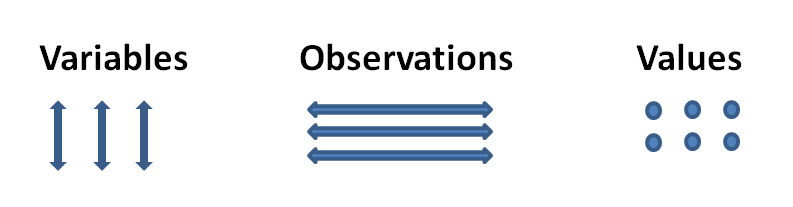
\includegraphics{01_var_obs_val.PNG}
\caption{}
\end{figure}

\subsection{\texorpdfstring{\textbf{readr }}{readr }}\label{readr}

\href{https://CRAN.R-project.org/package=readr}{\texttt{readr}}: Read
flat/tabular text files from disk (or a connection). readr has some
benefits over the base/utils version as smart column type parsing and
not automatically converting strings into factors.

\subsubsection{\texorpdfstring{\textbf{Examples
}}{Examples }}\label{examples}

\begin{itemize}
\tightlist
\item
  Here is an example of
  \href{http://archive.ics.uci.edu/ml/datasets/Credit+Approval}{credit
  card applications data set} from the
  \href{http://archive.ics.uci.edu/ml/index.html}{UCI Machine Learning
  Repository} using \texttt{readr}:
\end{itemize}

\begin{Shaded}
\begin{Highlighting}[]
\KeywordTok{library}\NormalTok{(readr)}
\NormalTok{cc_apps <-}\StringTok{ }\KeywordTok{read_csv}\NormalTok{(}\StringTok{"http://archive.ics.uci.edu/ml/machine-learning-databases/credit-screening/crx.data"}\NormalTok{, }\DataTypeTok{col_names =} \NormalTok{F)}
\KeywordTok{head}\NormalTok{(cc_apps)}
\end{Highlighting}
\end{Shaded}

\begin{verbatim}
## # A tibble: 6 × 16
##      X1    X2    X3    X4    X5    X6    X7    X8    X9   X10   X11   X12
##   <chr> <dbl> <dbl> <chr> <chr> <chr> <chr> <dbl> <chr> <chr> <chr> <chr>
## 1     b 30.83 0.000     u     g     w     v  1.25     t     t    01     f
## 2     a 58.67 4.460     u     g     q     h  3.04     t     t    06     f
## 3     a 24.50 0.500     u     g     q     h  1.50     t     f     0     f
## 4     b 27.83 1.540     u     g     w     v  3.75     t     t    05     t
## 5     b 20.17 5.625     u     g     w     v  1.71     t     f     0     f
## 6     b 32.08 4.000     u     g     m     v  2.50     t     f     0     t
## # ... with 4 more variables: X13 <chr>, X14 <chr>, X15 <int>, X16 <chr>
\end{verbatim}

\subsection{\texorpdfstring{\textbf{readxl }}{readxl }}\label{readxl}

\href{https://cran.r-project.org/package=readxl}{\texttt{readxl}}:
Import excel files into R. Supports `.xls' via the embedded `libxls' C
library (\url{http://sourceforge.net/projects/libxls/}) and `.xlsx' via
the embedded `RapidXML' C++ library
(\url{http://rapidxml.sourceforge.net}). Works on Windows, Mac and Linux
without external dependencies.

\subsubsection{\texorpdfstring{\textbf{Examples
}}{Examples }}\label{examples-1}

\begin{itemize}
\tightlist
\item
  Here is an example from the
  \href{http://archive.ics.uci.edu/ml/datasets/default+of+credit+card+clients}{default
  of credit card clients data set} from the
  \href{http://archive.ics.uci.edu/ml/index.html}{UCI Machine Learning
  Repository} using \texttt{readxl}:
\end{itemize}

\begin{Shaded}
\begin{Highlighting}[]
\CommentTok{# download the excel file first from the link}
\KeywordTok{library}\NormalTok{(readxl)}
\NormalTok{default_cc <-}\StringTok{ }\KeywordTok{read_excel}\NormalTok{(}\StringTok{"default of credit card clients.xls"}\NormalTok{)}

\CommentTok{# alternative reading from a URL}
\KeywordTok{require}\NormalTok{(RCurl)}
\KeywordTok{require}\NormalTok{(gdata)}
\NormalTok{url <-}\StringTok{ "http://archive.ics.uci.edu/ml/machine-learning-databases/00350/default%20of%20credit%20card%20clients.xls"}
\NormalTok{default_cc <-}\StringTok{ }\KeywordTok{read.xls}\NormalTok{(url)}

\KeywordTok{head}\NormalTok{(default_cc)}
\end{Highlighting}
\end{Shaded}

\begin{verbatim}
##    X        X1  X2        X3       X4  X5    X6    X7    X8    X9   X10
## 1 ID LIMIT_BAL SEX EDUCATION MARRIAGE AGE PAY_0 PAY_2 PAY_3 PAY_4 PAY_5
## 2  1     20000   2         2        1  24     2     2    -1    -1    -2
## 3  2    120000   2         2        2  26    -1     2     0     0     0
## 4  3     90000   2         2        2  34     0     0     0     0     0
## 5  4     50000   2         2        1  37     0     0     0     0     0
## 6  5     50000   1         2        1  57    -1     0    -1     0     0
##     X11       X12       X13       X14       X15       X16       X17
## 1 PAY_6 BILL_AMT1 BILL_AMT2 BILL_AMT3 BILL_AMT4 BILL_AMT5 BILL_AMT6
## 2    -2      3913      3102       689         0         0         0
## 3     2      2682      1725      2682      3272      3455      3261
## 4     0     29239     14027     13559     14331     14948     15549
## 5     0     46990     48233     49291     28314     28959     29547
## 6     0      8617      5670     35835     20940     19146     19131
##        X18      X19      X20      X21      X22      X23
## 1 PAY_AMT1 PAY_AMT2 PAY_AMT3 PAY_AMT4 PAY_AMT5 PAY_AMT6
## 2        0      689        0        0        0        0
## 3        0     1000     1000     1000        0     2000
## 4     1518     1500     1000     1000     1000     5000
## 5     2000     2019     1200     1100     1069     1000
## 6     2000    36681    10000     9000      689      679
##                            Y
## 1 default payment next month
## 2                          1
## 3                          1
## 4                          0
## 5                          0
## 6                          0
\end{verbatim}

\section{\texorpdfstring{\textbf{Hierarchical
Data}}{Hierarchical Data}}\label{hierarchical-data}

Hierarchical Data is a tree-structure data format such as
\href{https://en.wikipedia.org/wiki/XML}{XML},
\href{https://en.wikipedia.org/wiki/HTML}{HTML},
\href{https://en.wikipedia.org/wiki/JSON}{JSON}. Popular methods for
accessing this data are known as \textbf{web scraping} or \textbf{web
data mining} when the goal is to parse data on a web page into a
analysis-ready format such as a data frame.

\subsection{\texorpdfstring{\textbf{jsonlite
}}{jsonlite }}\label{jsonlite}

\href{https://CRAN.R-project.org/package=jsonlite}{\texttt{jsonlite}}: A
fast JSON parser and generator optimized for statistical data and the
web.

\subsubsection{\texorpdfstring{\textbf{Examples
}}{Examples }}\label{examples-2}

TBD

\subsection{\texorpdfstring{\textbf{xml2 }}{xml2 }}\label{xml2}

\href{https://CRAN.R-project.org/package=xml2}{\texttt{xml2}}: Work with
XML files using a simple, consistent interface. Built on top of the
`libxml2' C library.

\subsubsection{\texorpdfstring{\textbf{Examples
}}{Examples }}\label{examples-3}

TBD

\subsection{\texorpdfstring{\textbf{rvest }}{rvest }}\label{rvest}

\href{https://CRAN.R-project.org/package=rvest}{\texttt{rvest}}:
Wrappers around the `xml2' and `httr' packages to make it easy to
download, then manipulate, HTML and XML.

\subsubsection{\texorpdfstring{\textbf{Examples
}}{Examples }}\label{examples-4}

TBD

\section{\texorpdfstring{\textbf{Relational
Data}}{Relational Data}}\label{relational-data}

\href{https://en.wikipedia.org/wiki/Relational_database}{Relational
Data} consists of a collection of data items (tables) organized as a set
based on the data contents and its relation.

\subsection{\texorpdfstring{\textbf{DBI}}{DBI}}\label{dbi}

\href{https://CRAN.R-project.org/package=DBI}{\texttt{DBI}}: A database
interface definition for communication between R and relational database
management systems. All classes in this package are virtual and need to
be extended by the various R/DBMS implementations.

\subsubsection{\texorpdfstring{\textbf{Examples
}}{Examples }}\label{examples-5}

TBD

\subsection{\texorpdfstring{\textbf{RMySQL }}{RMySQL }}\label{rmysql}

\href{https://CRAN.R-project.org/package=RMySQL}{\texttt{RMySQL}}:
Implements `DBI' Interface to `MySQL' and `MariaDB' Databases.

\subsubsection{\texorpdfstring{\textbf{Examples
}}{Examples }}\label{examples-6}

TBD

\subsubsection{\texorpdfstring{\textbf{RPostgreSQL
}}{RPostgreSQL }}\label{rpostgresql}

\href{https://cran.r-project.org/package=RPostgreSQL}{\texttt{RPostgreSQL}}:Database
interface and PostgreSQL driver for R This package provides a Database
Interface (DBI) compliant driver for R to access PostgreSQL database
systems. In order to build and install this package from source,
PostgreSQL itself must be present your system to provide PostgreSQL
functionality via its libraries and header files. These files are
provided as postgresql-devel package under some Linux distributions. On
Microsoft Windows system the attached libpq library source will be used.
A wiki and issue tracking system for the package are available at Google
Code at \url{https://code.google.com/p/rpostgresql/}

\subsubsection{\texorpdfstring{\textbf{Examples
}}{Examples }}\label{examples-7}

TBD

\section{\texorpdfstring{\textbf{Distributed
Data}}{Distributed Data}}\label{distributed-data}

Distributed Data consists of non-relational formats with quick access to
data over a large number of nodes (data spread over many different
computers).

\subsection{\texorpdfstring{\textbf{sparklyr
}}{sparklyr }}\label{sparklyr}

\href{http://spark.rstudio.com/}{\texttt{sparklyr}}: Filter and
aggregate Spark datasets then bring them into R for analysis and
visualization.

\subsubsection{\texorpdfstring{\textbf{Examples
}}{Examples }}\label{examples-8}

TBD

\section{\texorpdfstring{\textbf{Additional Import
Methods}}{Additional Import Methods}}\label{additional-import-methods}

\textbf{Different Data Formats}: The R programming language and
environment is continuously increasing its capacity with new packages to
work with different types of proprietory data formats from statistical
software packages that are used on industry teams.

\subsection{\texorpdfstring{\textbf{haven }}{haven }}\label{haven}

\href{https://CRAN.R-project.org/package=haven}{\texttt{haven}}: Import
and Export `SPSS', `Stata' and `SAS' Files.

\subsubsection{\texorpdfstring{\textbf{Examples
}}{Examples }}\label{examples-9}

Here is an example from
\href{http://www.businessandeconomics.mq.edu.au/our_departments/Applied_Finance_and_Actuarial_Studies/research/books/GLMsforInsuranceData/data_sets}{Macquarie
University data repository for the applied finance and actuarial
studies} of importing a \href{http://www.sas.com/en_us/home.html}{SAS}
data set:

\begin{Shaded}
\begin{Highlighting}[]
\KeywordTok{library}\NormalTok{(haven)}
\NormalTok{claims <-}\StringTok{ }\KeywordTok{read_sas}\NormalTok{(}\StringTok{"http://www.businessandeconomics.mq.edu.au/our_departments/Applied_Finance_and_Actuarial_Studies/acst_docs/glms_for_insurance_data/data/claims_sas_miner.sas7bdat"}\NormalTok{)}
\KeywordTok{head}\NormalTok{(claims)}
\end{Highlighting}
\end{Shaded}

\begin{verbatim}
## # A tibble: 6 × 33
##          ID KIDSDRIV   PLCYDATE TRAVTIME    CAR_USE POLICYNO BLUEBOOK
##       <chr>    <dbl>     <date>    <dbl>      <chr>    <dbl>    <dbl>
## 1 100058542        0 1996-03-17 17.09181    Private 36292520     9860
## 2 100093408        0 1993-07-26 17.98656    Private 31958061     1500
## 3 100208113        0 1994-06-06 47.00727 Commercial 42433312    30460
## 4 100237269        0 1999-01-19 31.24381    Private 49896544    16580
## 5  10042968        0 1999-05-18 13.96243 Commercial 79298192    23030
## 6 100737644        0 1996-02-28 45.79204    Private 43393435    20730
## # ... with 26 more variables: INITDATE <date>, RETAINED <dbl>,
## #   NPOLICY <dbl>, CAR_TYPE <chr>, RED_CAR <chr>, OLDCLAIM <dbl>,
## #   CLM_FREQ <dbl>, REVOLKED <chr>, MVR_PTS <dbl>, CLM_AMT <dbl>,
## #   CLM_DATE <date>, CLM_FLAG <chr>, BIRTH <date>, AGE <dbl>,
## #   HOMEKIDS <dbl>, YOJ <dbl>, INCOME <dbl>, GENDER <chr>, MARRIED <chr>,
## #   PARENT1 <chr>, JOBCLASS <chr>, MAX_EDUC <chr>, HOME_VAL <dbl>,
## #   SAMEHOME <dbl>, DENSITY <chr>, YEARQTR <chr>
\end{verbatim}

\subsection{\texorpdfstring{\textbf{foreign }}{foreign }}\label{foreign}

\href{https://CRAN.R-project.org/package=foreign}{\texttt{foreign}}:
Functions for reading and writing data stored by some versions of Epi
Info, Minitab, S, SAS, SPSS, Stata, Systat and Weka and for reading and
writing some dBase files.

\subsubsection{\texorpdfstring{\textbf{Examples
}}{Examples }}\label{examples-10}

TBD

\subsection{\texorpdfstring{\textbf{\emph{Zipped Data}
}}{Zipped Data }}\label{zipped-data}

\textbf{Accessing Zipped Data files}:
\href{https://en.wikipedia.org/wiki/Zip_(file_format)}{Zip archives} are
actually more a `filesystem' with content, meta data, and/or
documentation.

\begin{enumerate}
\def\labelenumi{\arabic{enumi}.}
\tightlist
\item
  Create a temp file. file name (eg tempfile())
\item
  Use download.file() to download the file into the temp object that is
  being reserved for the file
\item
  Use unzip() to extract the target file from temp file by reading the
  meta data on what specific data set you want which is contained in the
  zip file
\item
  Remove the temp file via unlink()
\end{enumerate}

\begin{Shaded}
\begin{Highlighting}[]
\NormalTok{temp <-}\StringTok{ }\KeywordTok{tempfile}\NormalTok{()}
\KeywordTok{download.file}\NormalTok{(}\StringTok{"http://archive.ics.uci.edu/ml/machine-learning-databases/00222/bank.zip"}\NormalTok{,temp)}
\KeywordTok{unzip}\NormalTok{(temp, }\StringTok{"bank.csv"}\NormalTok{)}
\NormalTok{bank_marketing <-}\StringTok{ }\KeywordTok{read.csv}\NormalTok{(}\StringTok{"bank.csv"}\NormalTok{, }\DataTypeTok{sep=}\StringTok{";"}\NormalTok{) }\CommentTok{# sometimes its the default}
\KeywordTok{unlink}\NormalTok{(temp)}
\KeywordTok{head}\NormalTok{(bank_marketing)}
\end{Highlighting}
\end{Shaded}

\begin{verbatim}
##   age         job marital education default balance housing loan  contact
## 1  30  unemployed married   primary      no    1787      no   no cellular
## 2  33    services married secondary      no    4789     yes  yes cellular
## 3  35  management  single  tertiary      no    1350     yes   no cellular
## 4  30  management married  tertiary      no    1476     yes  yes  unknown
## 5  59 blue-collar married secondary      no       0     yes   no  unknown
## 6  35  management  single  tertiary      no     747      no   no cellular
##   day month duration campaign pdays previous poutcome  y
## 1  19   oct       79        1    -1        0  unknown no
## 2  11   may      220        1   339        4  failure no
## 3  16   apr      185        1   330        1  failure no
## 4   3   jun      199        4    -1        0  unknown no
## 5   5   may      226        1    -1        0  unknown no
## 6  23   feb      141        2   176        3  failure no
\end{verbatim}

\chapter{Tidy}\label{tidy}

\section{\texorpdfstring{\textbf{Introduction}}{Introduction}}\label{introduction-2}

Reshaping the data is an important (if necessary) step to exploratory
data analysis and preparatory data cleaning for modeling or creating
specialized visualization. Further concepts about \emph{tidy data} can
be found in this paper
\href{http://vita.had.co.nz/papers/tidy-data.pdf}{Tidy Data}.

The principles of tidy data are:

\begin{enumerate}
\def\labelenumi{\arabic{enumi}.}
\tightlist
\item
  Each variable forms a column
\item
  Each observation forms a row
\item
  Each type of observational unit forms a table
\end{enumerate}

\subsection{\texorpdfstring{\textbf{tidyr }}{tidyr }}\label{tidyr}

\begin{itemize}
\tightlist
\item
  \href{https://cran.r-project.org/web/packages/tidyr/index.html}{\texttt{tidyr}}:
  An evolution of `reshape2'. It's designed specifically for data
  tidying (not general reshaping or aggregating) and works well with
  `dplyr' data pipelines. Tidy data complements R's vectorized
  operations. R will automatically preserve observations as you
  manipulate variables. No other format works as intuitively with R.
\end{itemize}

\subsubsection{\texorpdfstring{\textbf{Examples
}}{Examples }}\label{examples-11}

\begin{Shaded}
\begin{Highlighting}[]
\KeywordTok{library}\NormalTok{(tidyr)}
\KeywordTok{library}\NormalTok{(insuranceData)}
\KeywordTok{library}\NormalTok{(magrittr)}
\KeywordTok{data}\NormalTok{(}\StringTok{"AutoBi"}\NormalTok{)}
\KeywordTok{head}\NormalTok{(AutoBi)}
\end{Highlighting}
\end{Shaded}

\begin{verbatim}
##   CASENUM ATTORNEY CLMSEX MARITAL CLMINSUR SEATBELT CLMAGE   LOSS
## 1       5        1      1      NA        2        1     50 34.940
## 2      13        2      2       2        1        1     28 10.892
## 3      66        2      1       2        2        1      5  0.330
## 4      71        1      1       1        2        2     32 11.037
## 5      96        2      1       4        2        1     30  0.138
## 6      97        1      2       1        2        1     35  0.309
\end{verbatim}

\begin{Shaded}
\begin{Highlighting}[]
\CommentTok{# create an interaction column}
\NormalTok{g <-}\StringTok{ }\NormalTok{AutoBi %>%}\StringTok{  }\KeywordTok{unite}\NormalTok{(}\DataTypeTok{col =} \NormalTok{MARITAL_CLMAGE, MARITAL, CLMAGE, }\DataTypeTok{sep =} \StringTok{"*"}\NormalTok{)}

\KeywordTok{head}\NormalTok{(g)}
\end{Highlighting}
\end{Shaded}

\begin{verbatim}
##   CASENUM ATTORNEY CLMSEX MARITAL_CLMAGE CLMINSUR SEATBELT   LOSS
## 1       5        1      1          NA*50        2        1 34.940
## 2      13        2      2           2*28        1        1 10.892
## 3      66        2      1            2*5        2        1  0.330
## 4      71        1      1           1*32        2        2 11.037
## 5      96        2      1           4*30        2        1  0.138
## 6      97        1      2           1*35        2        1  0.309
\end{verbatim}

Not all data that needs to be \emph{tidied} comes in ``long'' format
(i.e.~the \texttt{spread()} function), so this data set below is put
into tidy or cleaned format using base R functions and general
manipulation. This data set has its observations stored in the row names
field, delimited with a semicolon ``;''. The original column contains a
mis-transformed value for the population density metric. The only
variables' names are also a concatenation of the entire data set's
column names delimited with a period ``.''.

\begin{itemize}
\tightlist
\item
  \href{http://www.businessandeconomics.mq.edu.au/our_departments/Applied_Finance_and_Actuarial_Studies/acst_docs/glms_for_insurance_data/data/third_party_claims.txt}{Data
  dictionary}
\item
  \href{http://www.businessandeconomics.mq.edu.au/our_departments/Applied_Finance_and_Actuarial_Studies/acst_docs/glms_for_insurance_data/data/Third_party_claims.xls}{Original
  source data used in the insuranceData package}
\end{itemize}

\begin{Shaded}
\begin{Highlighting}[]
\KeywordTok{library}\NormalTok{(insuranceData)}
\KeywordTok{library}\NormalTok{(magrittr)}
\KeywordTok{data}\NormalTok{(}\StringTok{"Thirdparty"}\NormalTok{)}

\KeywordTok{head}\NormalTok{(Thirdparty) }\CommentTok{# rownames have column values}
\end{Highlighting}
\end{Shaded}

\begin{verbatim}
##                                         lga.sd.claims.accidents.ki.population.pop_density
## ASHFIELD;1;1103;2304;920;124850;0                                                  499001
## AUBURN;1;1939;2660;1465;143500;0                                                   148379
## BANKSTOWN;1;4339;7381;3864;470700;0                                                205407
## BAULKHAMHILLS;1;1491;3217;1554;311300;0                                             25879
## BLACKTOWN;1;3801;6655;4175;584900;0                                                 81222
## BOTANY;1;387;2013;854;106350;0                                                     178143
\end{verbatim}

\begin{Shaded}
\begin{Highlighting}[]
\NormalTok{cols =}\StringTok{ }\KeywordTok{strsplit}\NormalTok{(}\KeywordTok{colnames}\NormalTok{(Thirdparty) , }\StringTok{"."} \NormalTok{, }\DataTypeTok{fixed=}\NormalTok{T)   }\CommentTok{# a new vector to use later }
\KeywordTok{dput}\NormalTok{(}\KeywordTok{unlist}\NormalTok{(cols))}
\end{Highlighting}
\end{Shaded}

\begin{verbatim}
## c("lga", "sd", "claims", "accidents", "ki", "population", "pop_density"
## )
\end{verbatim}

\begin{Shaded}
\begin{Highlighting}[]
\NormalTok{rows2df <-}\StringTok{ }\KeywordTok{sapply}\NormalTok{(}\KeywordTok{rownames}\NormalTok{(Thirdparty), strsplit, }\StringTok{";"}\NormalTok{, }\DataTypeTok{USE.NAMES =} \OtherTok{FALSE}\NormalTok{)}

\NormalTok{tidy_3PD <-}\StringTok{ }\KeywordTok{data.frame}\NormalTok{(}\KeywordTok{matrix}\NormalTok{(}\KeywordTok{unlist}\NormalTok{(rows2df), }\DataTypeTok{nrow =} \KeywordTok{nrow}\NormalTok{(Thirdparty), }\DataTypeTok{byrow=}\NormalTok{T))}
\KeywordTok{colnames}\NormalTok{(tidy_3PD) <-}\StringTok{ }\KeywordTok{c}\NormalTok{(}\StringTok{"lga"}\NormalTok{, }\StringTok{"sd"}\NormalTok{, }\StringTok{"claims"}\NormalTok{, }\StringTok{"accidents"}\NormalTok{, }\StringTok{"ki"}\NormalTok{, }\StringTok{"population"}\NormalTok{,}
\StringTok{"pop_density"}\NormalTok{)}
\NormalTok{tidy_3PD$pop_density <-}\StringTok{ }\NormalTok{Thirdparty$lga.sd.claims.accidents.ki.population.pop_density /}\StringTok{ }\DecValTok{1000000}

\KeywordTok{head}\NormalTok{(tidy_3PD)}
\end{Highlighting}
\end{Shaded}

\begin{verbatim}
##             lga sd claims accidents   ki population pop_density
## 1      ASHFIELD  1   1103      2304  920     124850    0.499001
## 2        AUBURN  1   1939      2660 1465     143500    0.148379
## 3     BANKSTOWN  1   4339      7381 3864     470700    0.205407
## 4 BAULKHAMHILLS  1   1491      3217 1554     311300    0.025879
## 5     BLACKTOWN  1   3801      6655 4175     584900    0.081222
## 6        BOTANY  1    387      2013  854     106350    0.178143
\end{verbatim}

\begin{center}\rule{0.5\linewidth}{\linethickness}\end{center}

\emph{Every variable forms a column and every observation forms a row
which makes for a table!}

\chapter{Transform}\label{transform}

\section{\texorpdfstring{\textbf{Introduction
}}{Introduction }}\label{introduction-3}

Transforming cleaned data to create summaries and aggregations is an
common part of the data analysis process along with extracting out data
to create new features. With SQL-like commands you can answer numerous
questions in the exploratory phase of a analysis prior to building a
model with \texttt{dplyr}.

\subsection{\texorpdfstring{\textbf{dplyr }}{dplyr }}\label{dplyr}

\href{https://cran.r-project.org/web/packages/dplyr/index.html}{\texttt{dplyr}}:
A fast, consistent tool for working with data frame like objects, both
in memory and out of memory.

\subsubsection{\texorpdfstring{\textbf{Examples
}}{Examples }}\label{examples-12}

\begin{Shaded}
\begin{Highlighting}[]
\KeywordTok{library}\NormalTok{(dplyr)}
\KeywordTok{library}\NormalTok{(insuranceData)}
\KeywordTok{library}\NormalTok{(magrittr)}
\KeywordTok{data}\NormalTok{(}\StringTok{"AutoBi"}\NormalTok{)}

\CommentTok{# summary of loss by whether or not the claimant was wearing a seatbelt/child restraint}

\NormalTok{AutoBi %>%}\StringTok{ }\KeywordTok{group_by}\NormalTok{(SEATBELT, MARITAL) %>%}\StringTok{ }
\StringTok{           }\KeywordTok{summarise}\NormalTok{(}\DataTypeTok{mLOSS =} \KeywordTok{median}\NormalTok{(LOSS))}
\end{Highlighting}
\end{Shaded}

\begin{verbatim}
## Source: local data frame [10 x 3]
## Groups: SEATBELT [?]
## 
##    SEATBELT MARITAL mLOSS
##       <int>   <int> <dbl>
## 1         1       1 2.641
## 2         1       2 1.780
## 3         1       3 1.703
## 4         1       4 3.845
## 5         1      NA 3.120
## 6         2       1 3.919
## 7         2       2 2.328
## 8        NA       1 1.985
## 9        NA       2 1.433
## 10       NA      NA 2.364
\end{verbatim}

\chapter{Visualization}\label{viz}

\section{\texorpdfstring{\textbf{Introduction}}{Introduction}}\label{introduction-4}

Data Visualization allows for the effective translation of data and
processes into business applicable decisions that can explain key
metrics. Ploting data prior to analysis can give key insights on
variables and distributions.

\section{\texorpdfstring{\textbf{Exploratory
Visualization}}{Exploratory Visualization}}\label{exploratory-visualization}

Exploratory visualization involoves learning descriptive details prior
to modeling efforts. Preemptive results from visualizing distributions
can lead to more informed approachs in variable transformation, error
distribution selection, parameter tunning.

\subsection{\texorpdfstring{\textbf{ggplot2}}{ggplot2}}\label{ggplot2}

\href{https://cran.r-project.org/web/packages/ggplot2/index.html}{\texttt{ggplot2}}:
An implementation of the grammar of graphics in R. It combines the
advantages of both base and lattice graphics: conditioning and shared
axes are handled automatically, and you can still build up a plot step
by step from multiple data sources. It also implements a sophisticated
multidimensional conditioning system and a consistent interface to map
data to aesthetic attributes.

\subsubsection{\texorpdfstring{\textbf{Examples:}}{Examples:}}\label{examples-13}

\begin{Shaded}
\begin{Highlighting}[]
\KeywordTok{library}\NormalTok{(ggplot2)}
\KeywordTok{library}\NormalTok{(insuranceData)}
\KeywordTok{data}\NormalTok{(}\StringTok{"AutoClaims"}\NormalTok{)}
\KeywordTok{head}\NormalTok{(AutoClaims)}
\end{Highlighting}
\end{Shaded}

\begin{verbatim}
##      STATE CLASS GENDER AGE    PAID
## 1 STATE 14   C6       M  97 1134.44
## 2 STATE 15   C6       M  96 3761.24
## 3 STATE 15   C11      M  95 7842.31
## 4 STATE 15   F6       F  95 2384.67
## 5 STATE 15   F6       M  95  650.00
## 6 STATE 15   F6       M  95  391.12
\end{verbatim}

\begin{Shaded}
\begin{Highlighting}[]
\NormalTok{g <-}\StringTok{ }\KeywordTok{ggplot}\NormalTok{(AutoClaims, }\KeywordTok{aes}\NormalTok{(}\DataTypeTok{x =} \NormalTok{AGE)) +}
\StringTok{            }\KeywordTok{geom_bar}\NormalTok{() +}
\StringTok{            }\KeywordTok{facet_grid}\NormalTok{(. ~}\StringTok{ }\NormalTok{GENDER)}
\NormalTok{g}
\end{Highlighting}
\end{Shaded}

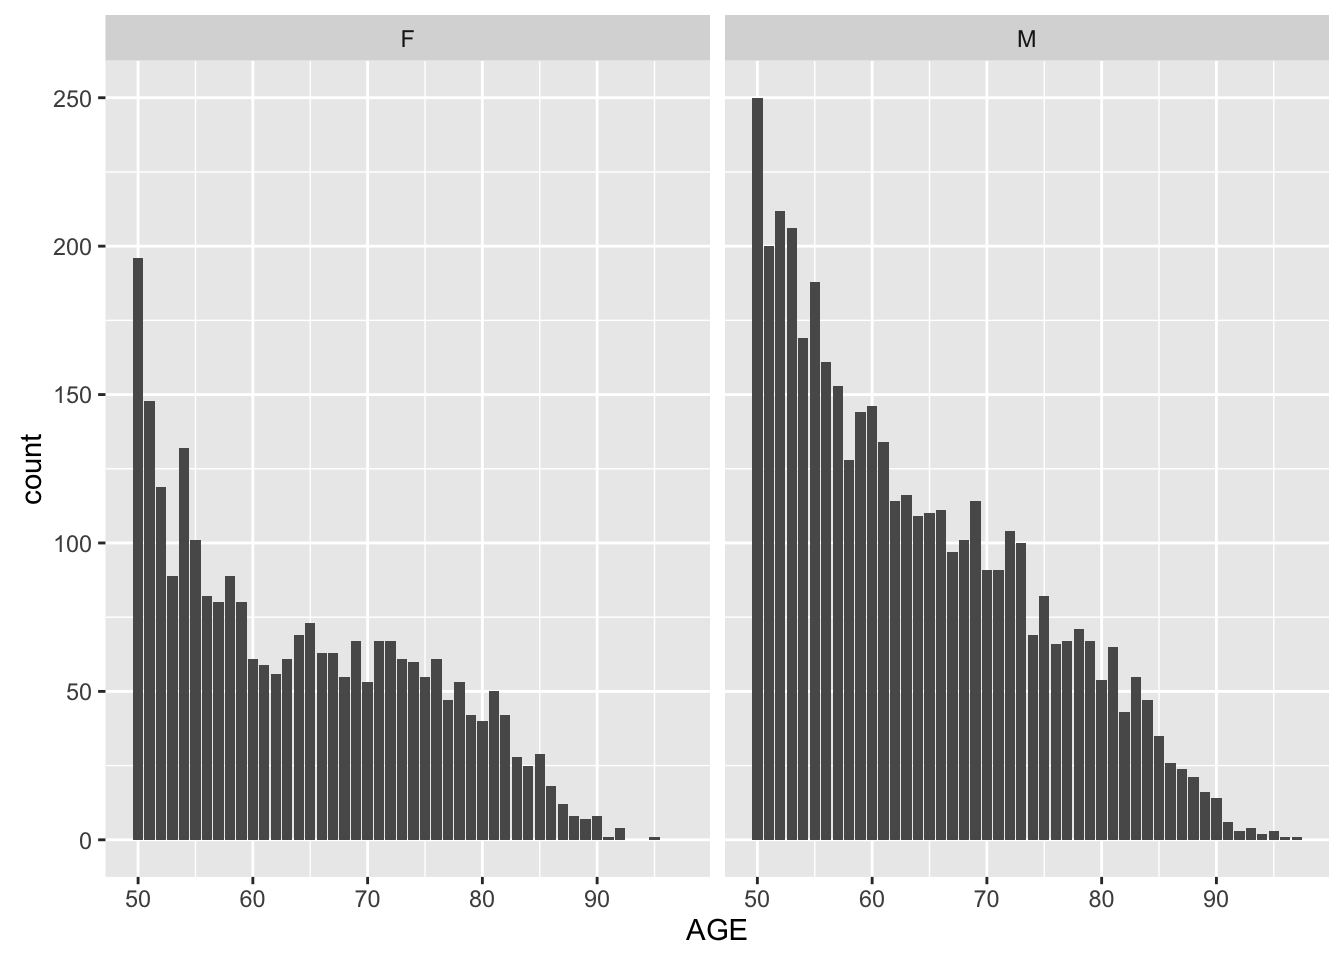
\includegraphics{r4fintech_files/figure-latex/ggplot2-exp1-1.pdf}

\begin{center}\rule{0.5\linewidth}{\linethickness}\end{center}

\begin{Shaded}
\begin{Highlighting}[]
\KeywordTok{library}\NormalTok{(ggplot2)}
\KeywordTok{library}\NormalTok{(insuranceData)}


\NormalTok{g2 <-}\StringTok{ }\KeywordTok{ggplot}\NormalTok{(AutoClaims, }\KeywordTok{aes}\NormalTok{(}\DataTypeTok{x =} \NormalTok{AGE, }\DataTypeTok{y =} \NormalTok{PAID, }\DataTypeTok{color =} \NormalTok{GENDER)) +}
\StringTok{            }\KeywordTok{geom_point}\NormalTok{() +}
\StringTok{            }\KeywordTok{geom_text}\NormalTok{(}\KeywordTok{aes}\NormalTok{(}\DataTypeTok{label =} \NormalTok{STATE)) +}
\StringTok{            }\KeywordTok{theme_classic}\NormalTok{()}
\NormalTok{g2}
\end{Highlighting}
\end{Shaded}

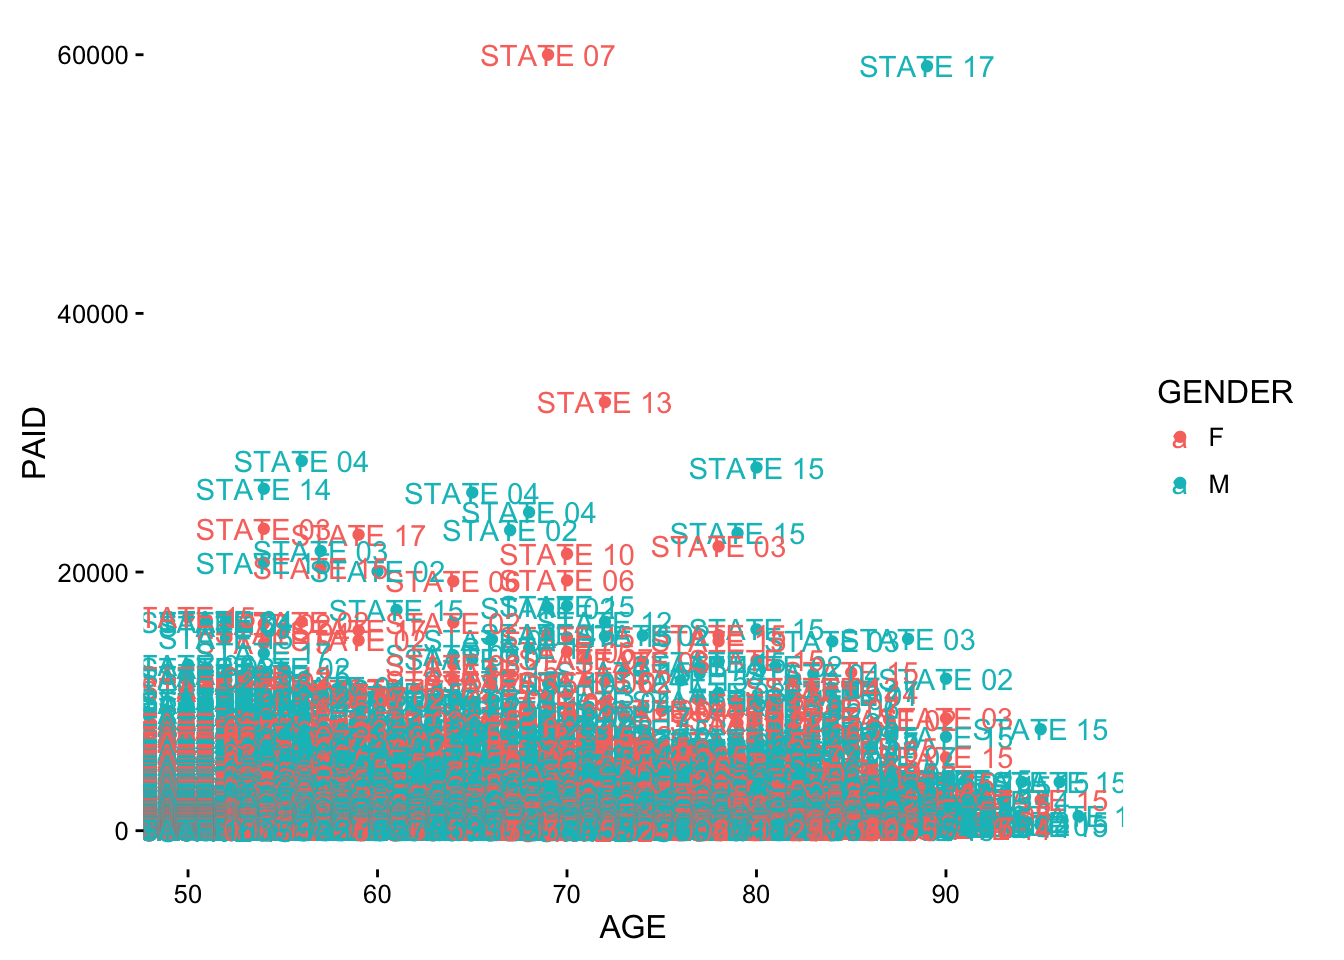
\includegraphics{r4fintech_files/figure-latex/ggplot2-exp2-1.pdf}

\section{\texorpdfstring{\textbf{Interactive
Visualization}}{Interactive Visualization}}\label{interactive-visualization}

\subsection{\texorpdfstring{\textbf{plotly}}{plotly}}\label{plotly}

\href{https://cran.r-project.org/web/packages/plotly/index.html}{\texttt{plotly}}:
Easily translate `ggplot2' graphs to an interactive web-based version
and/or create custom web-based visualizations directly from R. Once
uploaded to a `plotly' account, `plotly' graphs (and the data behind
them) can be viewed and modified in a web browser.

\subsubsection{\texorpdfstring{\textbf{Examples}}{Examples}}\label{examples-14}

\begin{Shaded}
\begin{Highlighting}[]
\KeywordTok{suppressPackageStartupMessages}\NormalTok{(}\KeywordTok{library}\NormalTok{(plotly))}
\KeywordTok{library}\NormalTok{(insuranceData)}
\KeywordTok{data}\NormalTok{(}\StringTok{"AutoCollision"}\NormalTok{)}
\KeywordTok{head}\NormalTok{(AutoCollision)}
\end{Highlighting}
\end{Shaded}

\begin{verbatim}
##   Age Vehicle_Use Severity Claim_Count
## 1   A    Pleasure   250.48          21
## 2   A  DriveShort   274.78          40
## 3   A   DriveLong   244.52          23
## 4   A    Business   797.80           5
## 5   B    Pleasure   213.71          63
## 6   B  DriveShort   298.60         171
\end{verbatim}

\begin{Shaded}
\begin{Highlighting}[]
\KeywordTok{plot_ly}\NormalTok{(AutoCollision, }\DataTypeTok{x =} \NormalTok{Severity, }\DataTypeTok{y =} \NormalTok{Claim_Count, }\DataTypeTok{mode =} \StringTok{"markers"}\NormalTok{, }
        \DataTypeTok{color =} \NormalTok{Severity, }\DataTypeTok{size =} \NormalTok{Severity)}
\end{Highlighting}
\end{Shaded}

\hypertarget{htmlwidget-7c1f63ec90ec6edcb56c}{}

\section{\texorpdfstring{\textbf{Other visualization
packages}}{Other visualization packages}}\label{other-visualization-packages}

\begin{itemize}
\tightlist
\item
  \href{http://ramnathv.github.io/rCharts/}{rcharts}
\item
  \href{https://rstudio.github.io/leaflet/}{leaflet}
\item
  \href{http://ggvis.rstudio.com/}{ggvis}
\item
  \href{http://www.htmlwidgets.org/}{htmlwidget}
\item
  \href{https://cran.r-project.org/web/packages/googleVis/vignettes/googleVis_examples.html}{googleVis}
\end{itemize}

\chapter{Model}\label{model}

Build Models

\section{\texorpdfstring{\textbf{LM}}{LM}}\label{lm}

\begin{itemize}
\tightlist
\item
  \href{https://stat.ethz.ch/R-manual/R-devel/library/stats/html/lm.html}{\texttt{lm()}}:
  In statistics, the term linear model is used for drawing primary
  associations with a response (dependent variable) and covariate(s)
  (independent variable(s)) as a regression analysis technique.
  \href{https://en.wikipedia.org/wiki/Linear_model}{Source: Wikipedia}
\end{itemize}

\textbf{Examples:}

\begin{Shaded}
\begin{Highlighting}[]
\KeywordTok{library}\NormalTok{(insuranceData)}
\KeywordTok{data}\NormalTok{(}\StringTok{"AutoCollision"}\NormalTok{)}
\KeywordTok{head}\NormalTok{(AutoCollision)}
\end{Highlighting}
\end{Shaded}

\begin{verbatim}
##   Age Vehicle_Use Severity Claim_Count
## 1   A    Pleasure   250.48          21
## 2   A  DriveShort   274.78          40
## 3   A   DriveLong   244.52          23
## 4   A    Business   797.80           5
## 5   B    Pleasure   213.71          63
## 6   B  DriveShort   298.60         171
\end{verbatim}

\begin{Shaded}
\begin{Highlighting}[]
\NormalTok{fit <-}\StringTok{ }\KeywordTok{lm}\NormalTok{(Severity ~}\StringTok{ }\NormalTok{Vehicle_Use +}\StringTok{ }\NormalTok{Age +}\StringTok{ }\NormalTok{Claim_Count, }\DataTypeTok{data =} \NormalTok{AutoCollision)}
\KeywordTok{summary}\NormalTok{(fit)}
\end{Highlighting}
\end{Shaded}

\begin{verbatim}
## 
## Call:
## lm(formula = Severity ~ Vehicle_Use + Age + Claim_Count, data = AutoCollision)
## 
## Residuals:
##      Min       1Q   Median       3Q      Max 
## -130.430  -24.580   -1.353   23.368  274.270 
## 
## Coefficients:
##                        Estimate Std. Error t value Pr(>|t|)    
## (Intercept)            523.0303    51.1632  10.223 2.18e-09 ***
## Vehicle_UseDriveLong  -150.3807    50.6663  -2.968 0.007603 ** 
## Vehicle_UseDriveShort -198.6347    65.8048  -3.019 0.006786 ** 
## Vehicle_UsePleasure   -184.4265    40.9901  -4.499 0.000219 ***
## AgeB                  -105.7532    58.6628  -1.803 0.086521 .  
## AgeC                  -128.0870    65.4756  -1.956 0.064546 .  
## AgeD                  -137.4725    68.6554  -2.002 0.058992 .  
## AgeE                  -206.6701    70.2024  -2.944 0.008026 ** 
## AgeF                  -195.6402    97.7303  -2.002 0.059052 .  
## AgeG                  -183.3416    85.0540  -2.156 0.043476 *  
## AgeH                  -173.1478    71.6721  -2.416 0.025387 *  
## Claim_Count              0.1000     0.1468   0.681 0.503380    
## ---
## Signif. codes:  0 '***' 0.001 '**' 0.01 '*' 0.05 '.' 0.1 ' ' 1
## 
## Residual standard error: 81.67 on 20 degrees of freedom
## Multiple R-squared:  0.6472, Adjusted R-squared:  0.4532 
## F-statistic: 3.336 on 11 and 20 DF,  p-value: 0.009379
\end{verbatim}

\begin{Shaded}
\begin{Highlighting}[]
\CommentTok{# this is not the best model we could have constructed as the lm assumes the error distribution of the response to be normal (gaussian) - and for a severity model we know that a multiplicative Gamma distribution is more appropriate.}
\end{Highlighting}
\end{Shaded}

\section{\texorpdfstring{\textbf{GLM}}{GLM}}\label{glm}

\begin{itemize}
\tightlist
\item
  \href{http://www.statmethods.net/advstats/glm.html}{\texttt{glm()}}:
  In statistics, the generalized linear model (GLM) is a flexible
  generalization of ordinary linear regression that allows for response
  variables that have error distribution models other than a normal
  distribution. The GLM generalizes linear regression by allowing the
  linear model to be related to the response variable via a link
  function and by allowing the magnitude of the variance of each
  measurement to be a function of its predicted value.
  \href{https://en.wikipedia.org/wiki/Generalized_linear_model}{Source:
  Wikipedia}
\end{itemize}

\textbf{Examples: }

\begin{Shaded}
\begin{Highlighting}[]
\KeywordTok{library}\NormalTok{(insuranceData)}
\KeywordTok{data}\NormalTok{(}\StringTok{"AutoCollision"}\NormalTok{)}

\NormalTok{fit <-}\StringTok{ }\KeywordTok{glm}\NormalTok{(Severity ~}\StringTok{ }\NormalTok{Vehicle_Use +}\StringTok{ }\NormalTok{Age +}\StringTok{ }\NormalTok{Claim_Count, }\DataTypeTok{data =} \NormalTok{AutoCollision, }\DataTypeTok{family =} \KeywordTok{Gamma}\NormalTok{(}\DataTypeTok{link =} \StringTok{"inverse"}\NormalTok{))}
\KeywordTok{summary}\NormalTok{(fit)}
\end{Highlighting}
\end{Shaded}

\begin{verbatim}
## 
## Call:
## glm(formula = Severity ~ Vehicle_Use + Age + Claim_Count, family = Gamma(link = "inverse"), 
##     data = AutoCollision)
## 
## Deviance Residuals: 
##      Min        1Q    Median        3Q       Max  
## -0.36252  -0.07729   0.00388   0.06376   0.23788  
## 
## Coefficients:
##                         Estimate Std. Error t value Pr(>|t|)    
## (Intercept)            1.576e-03  1.939e-04   8.131 9.07e-08 ***
## Vehicle_UseDriveLong   1.206e-03  2.750e-04   4.388 0.000284 ***
## Vehicle_UseDriveShort  1.752e-03  3.760e-04   4.659 0.000151 ***
## Vehicle_UsePleasure    2.096e-03  2.671e-04   7.847 1.57e-07 ***
## AgeB                   7.881e-04  2.954e-04   2.668 0.014762 *  
## AgeC                   8.927e-04  3.411e-04   2.617 0.016503 *  
## AgeD                   9.567e-04  3.660e-04   2.614 0.016604 *  
## AgeE                   2.040e-03  4.331e-04   4.710 0.000134 ***
## AgeF                   1.381e-03  5.526e-04   2.500 0.021237 *  
## AgeG                   1.353e-03  4.600e-04   2.942 0.008068 ** 
## AgeH                   1.395e-03  3.902e-04   3.575 0.001894 ** 
## Claim_Count           -8.694e-08  9.419e-07  -0.092 0.927375    
## ---
## Signif. codes:  0 '***' 0.001 '**' 0.01 '*' 0.05 '.' 0.1 ' ' 1
## 
## (Dispersion parameter for Gamma family taken to be 0.02045281)
## 
##     Null deviance: 3.20647  on 31  degrees of freedom
## Residual deviance: 0.42585  on 20  degrees of freedom
## AIC: 335.24
## 
## Number of Fisher Scoring iterations: 4
\end{verbatim}

\begin{Shaded}
\begin{Highlighting}[]
\NormalTok{r_squared =}\StringTok{ }\DecValTok{1} \NormalTok{-}\StringTok{ }\NormalTok{( fit$deviance /}\StringTok{ }\NormalTok{fit$df.null ) }\CommentTok{# psuedo r2 for GLMs}

\NormalTok{r_squared }
\end{Highlighting}
\end{Shaded}

\begin{verbatim}
## [1] 0.9862631
\end{verbatim}

\begin{Shaded}
\begin{Highlighting}[]
\CommentTok{# this model explains much more variance now that the error distribution has been specified correctly}
\end{Highlighting}
\end{Shaded}

\begin{itemize}
\item
  \href{https://en.wikipedia.org/wiki/Exponential_family}{Probability
  distributions from the exponential family}

  \begin{enumerate}
  \def\labelenumi{\arabic{enumi}.}
  \tightlist
  \item
    Claim Counts: \textbf{Multiplicative Poisson} model forms fit due to
    the poisson distribution is invariant to meatures of time.
  \item
    Frequency: \textbf{Multiplicative Poisson} model forms fit due to
    the poisson distribution is invariant to meatures of time.
  \item
    Severity: \textbf{Multiplicative Gamma} model forms fit because the
    gamma distribution is invariant to measures of currency.
  \item
    Retension and New Business: \textbf{Binomial with logit} model form
    fits becasue the binomial distribution is invariant to measures of
    success or failure.
  \end{enumerate}
\end{itemize}

\section{\texorpdfstring{\textbf{GBM}}{GBM}}\label{gbm}

Gradient boosting is a machine learning technique for regression and
classification problems, which produces a prediction model in the form
of an ensemble of weak prediction models, typically decision trees. It
builds the model in a stage-wise fashion like other boosting methods do,
and it generalizes them by allowing optimization of an arbitrary
differentiable loss function.
\href{https://en.wikipedia.org/wiki/Gradient_boosting}{Source:
Wikipedia}

\begin{itemize}
\tightlist
\item
  \href{https://www.analyticsvidhya.com/blog/2016/02/complete-guide-parameter-tuning-gradient-boosting-gbm-python/}{Parameter
  tuning} is prudent in machine learning!
\end{itemize}

\textbf{Examples:}

\begin{Shaded}
\begin{Highlighting}[]
\KeywordTok{library}\NormalTok{(insuranceData)}
\KeywordTok{data}\NormalTok{(}\StringTok{"AutoCollision"}\NormalTok{)}
\KeywordTok{library}\NormalTok{(gbm)}

\CommentTok{# let's build a a GBM model which combines some weak learners into a strong learner as to boost the predictive power of those variables which contribute the most to the model}
\NormalTok{fit <-}\StringTok{ }\KeywordTok{gbm}\NormalTok{(Claim_Count ~}\StringTok{ }\NormalTok{Vehicle_Use +}\StringTok{ }\NormalTok{Age +}\StringTok{ }\NormalTok{Severity, }\DataTypeTok{data=}\NormalTok{AutoCollision, }\DataTypeTok{distribution =} \StringTok{"poisson"}\NormalTok{, }\DataTypeTok{n.trees =} \DecValTok{50}\NormalTok{, }\DataTypeTok{bag.fraction =} \FloatTok{0.8}\NormalTok{)}
\KeywordTok{summary}\NormalTok{(fit)}
\end{Highlighting}
\end{Shaded}

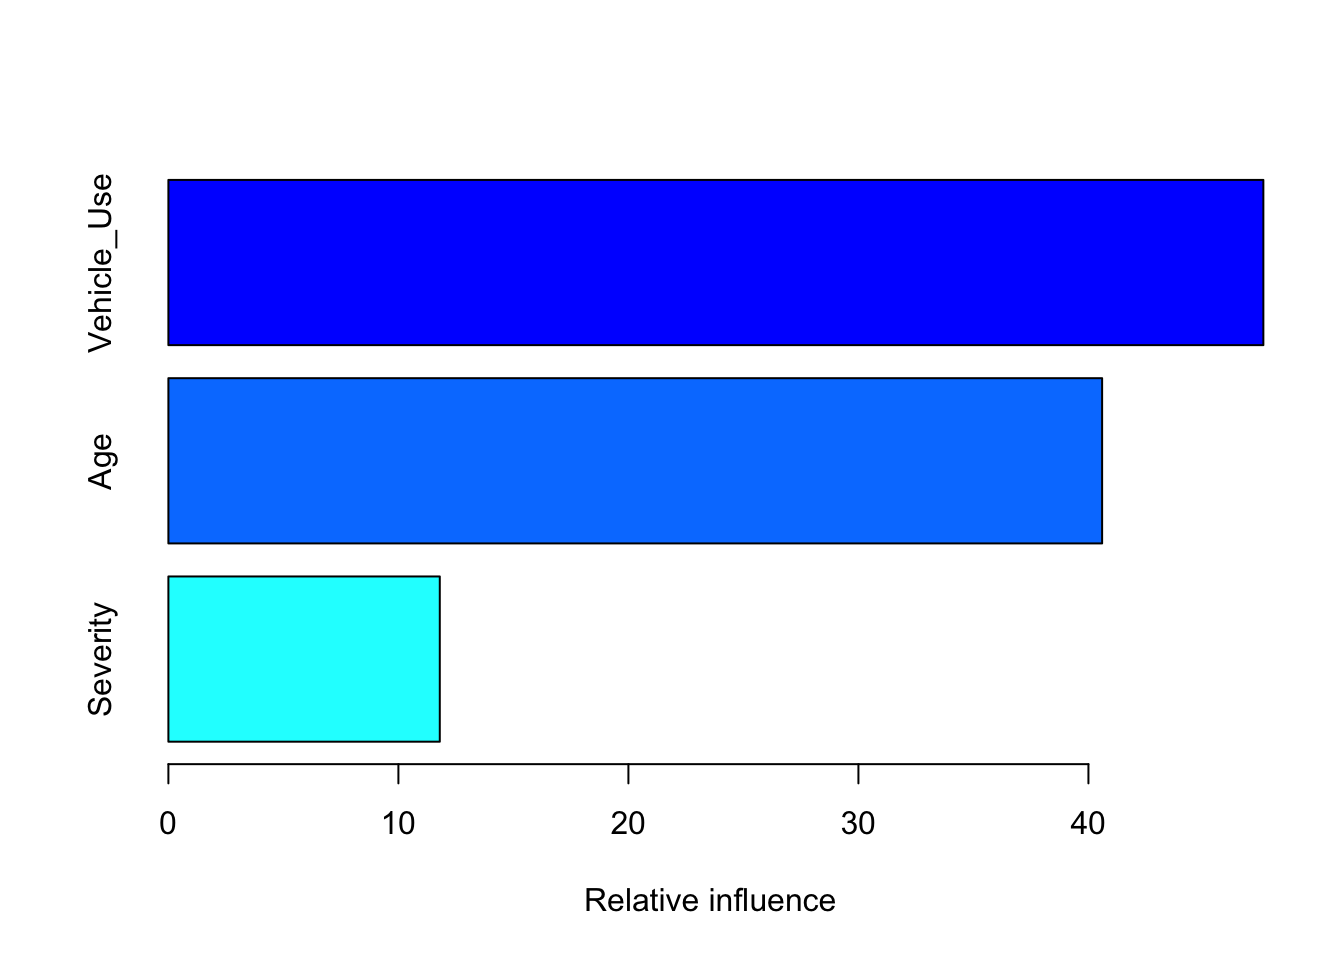
\includegraphics{r4fintech_files/figure-latex/gbm-exp1-1.pdf}

\begin{verbatim}
##                     var   rel.inf
## Age                 Age 46.741540
## Vehicle_Use Vehicle_Use 46.358522
## Severity       Severity  6.899939
\end{verbatim}

\section{\texorpdfstring{\textbf{Ensemble
learning}}{Ensemble learning}}\label{ensemble-learning}

In statistics and machine learning, ensemble methods use multiple
learning algorithms to obtain better predictive performance than could
be obtained from any of the constituent learning algorithms alone.
\href{https://en.wikipedia.org/wiki/Ensemble_learning}{Source:
Wikipedia}

\begin{itemize}
\tightlist
\item
  \href{http://blog.revolutionanalytics.com/2014/04/a-dive-into-h2o.html}{h2o
  / stacking}
\end{itemize}

\section{\texorpdfstring{\textbf{Additional Machine Learning
Techniques}}{Additional Machine Learning Techniques}}\label{additional-machine-learning-techniques}

\begin{itemize}
\tightlist
\item
  \href{https://xgboost.readthedocs.io/en/latest/}{\texttt{xgboost}}:
  Extreme Gradient Boosting, which is an efficient implementation of
  gradient boosting framework. This package is its R interface. The
  package includes efficient linear model solver and tree learning
  algorithms. The package can automatically do parallel computation on a
  single machine which could be more than 10 times faster than existing
  gradient boosting packages. It supports various objective functions,
  including regression, classification and ranking. The package is made
  to be extensible, so that users are also allowed to define their own
  objectives easily.
\item
  \href{https://cran.r-project.org/web/packages/TDboost/TDboost.pdf}{\texttt{TDboost}}:
  A boosted Tweedie compound Poisson model using the gradient boosting.
  It is capable of fitting a flexible nonlinear Tweedie compound Poisson
  model (or a gamma model) and capturing interactions among predictors.
\item
  \href{https://web.stanford.edu/~hastie/glmnet/glmnet_alpha.html}{\texttt{glmnet}:
  lasso, ridge, elasticnet}: Extremely efficient procedures for fitting
  the entire lasso (least absolute shrinkage and selection operator) or
  elastic-net regularization path for linear regression, logistic and
  multinomial regression models, Poisson regression and the Cox model.
  Two recent additions are the multiple-response Gaussian, and the
  grouped multinomial. The algorithm uses cyclical coordinate descent in
  a path-wise fashion.
\item
  \href{https://cran.r-project.org/web/packages/randomForest/randomForest.pdf}{\texttt{randomForest}}:
  Classification and regression based on a forest of trees using random
  inputs.
\item
  \href{http://www.statmethods.net/advstats/cluster.html}{K-means /
  K-mediods}: K Means Clustering is an unsupervised learning algorithm
  that tries to cluster data based on their similarity. Available in the
  base \texttt{stats} package
\end{itemize}

\chapter{Communicate}\label{communicate}

In Data Science our role is to be translators. We are tasked with
translating buisness-driven inquires to discovering implicit knowledge
from data and transforming knowledge into actionable results.

\section{\texorpdfstring{\textbf{Tools for Communication and
Reproducible
Research}}{Tools for Communication and Reproducible Research}}\label{tools-for-communication-and-reproducible-research}

\begin{itemize}
\item
  \href{http://yihui.name/knitr/}{\texttt{knitr}}: Provides a
  general-purpose tool for dynamic report generation in R using Literate
  Programming techniques.
\item
  \href{http://rmarkdown.rstudio.com/}{\texttt{rmarkdown}}: Convert R
  Markdown documents into a variety of formats (HTML, Word, PDF,
  Notebooks, Presentaions, dashboards).
\item
  \href{https://bookdown.org/yihui/bookdown/}{Bookdown (meta)}: Output
  formats and utilities for authoring books with R Markdown.
\item
  \href{http://shiny.rstudio.com/}{\texttt{shiny}}: Makes it incredibly
  easy to build interactive web applications with R. Automatic
  ``reactive'' binding between inputs and outputs and extensive
  pre-built widgets make it possible to build beautiful, responsive, and
  powerful applications with minimal effort.
\item
  \href{http://rmarkdown.rstudio.com/flexdashboard/}{\texttt{flexdashboard}}:
  Format for converting an R Markdown document to a grid oriented
  dashboard. The dashboard flexibly adapts the size of it's components
  to the containing web page.
\end{itemize}

\chapter{References}\label{references}

\begin{enumerate}
\def\labelenumi{\arabic{enumi}.}
\tightlist
\item
  Yihui Xie (NA). bookdown: Authoring Books with R Markdown. R package
  version 0.1.15. \url{https://github.com/rstudio/bookdown}
\item
  Hadley Wickham, Jim Hester and Romain Francois (2016). readr: Read
  Tabular Data. R package version 1.0.0.
  \url{https://CRAN.R-project.org/package=readr}
\item
  Hadley Wickham (2016). readxl: Read Excel Files. R package version
  0.1.1. \url{https://CRAN.R-project.org/package=readxl}
\item
  Jeroen Ooms (2014). The jsonlite Package: A Practical and Consistent
  Mapping Between JSON Data and R Objects. arXiv:1403.2805 {[}stat.CO{]}
  URL \url{http://arxiv.org/abs/1403.2805}.
\item
  Hadley Wickham and James Hester (2016). xml2: Parse XML. R package
  version 1.0.0. \url{https://CRAN.R-project.org/package=xml2}
\item
  Hadley Wickham (2016). rvest: Easily Harvest (Scrape) Web Pages. R
  package version 0.3.2. \url{https://CRAN.R-project.org/package=rvest}
\item
  R Special Interest Group on Databases (R-SIG-DB), Hadley Wickham and
  Kirill Müller (2016). DBI: R Database Interface. R package version
  0.5. \url{https://CRAN.R-project.org/package=DBI}
\item
  Jeroen Ooms, David James, Saikat DebRoy, Hadley Wickham and Jeffrey
  Horner (2016). RMySQL: Database Interface and `MySQL' Driver for R. R
  package version 0.10.9.
  \url{https://CRAN.R-project.org/package=RMySQL}
\item
  Joe Conway, Dirk Eddelbuettel, Tomoaki Nishiyama, Sameer Kumar Prayaga
  and Neil Tiffin (2016). RPostgreSQL: R interface to the PostgreSQL
  database system. R package version 0.4-1.
  \url{https://CRAN.R-project.org/package=RPostgreSQL}
\item
  Javier Luraschi, Kevin Ushey, JJ Allaire and The Apache Software
  Foundation (2016). sparklyr: R Interface to Apache Spark. R package
  version 0.4. \url{https://CRAN.R-project.org/package=sparklyr}
\item
  Hadley Wickham and Evan Miller (2016). haven: Import and Export
  `SPSS', `Stata' and `SAS' Files. R package version 1.0.0.
  \url{https://CRAN.R-project.org/package=haven}
\item
  R Core Team (2015). foreign: Read Data Stored by Minitab, S, SAS,
  SPSS, Stata, Systat, Weka, dBase, \ldots{}. R package version 0.8-66.
  \url{https://CRAN.R-project.org/package=foreign}
\end{enumerate}

\section{Session Info}\label{session-info}

\begin{verbatim}
## Session info --------------------------------------------------------------
\end{verbatim}

\begin{verbatim}
##  setting  value                       
##  version  R version 3.3.1 (2016-06-21)
##  system   x86_64, darwin13.4.0        
##  ui       X11                         
##  language (EN)                        
##  collate  en_US.UTF-8                 
##  tz       America/New_York            
##  date     2016-10-30
\end{verbatim}

\begin{verbatim}
## Packages ------------------------------------------------------------------
\end{verbatim}

\begin{verbatim}
##  package       * version  date       source                           
##  assertthat      0.1      2013-12-06 CRAN (R 3.3.0)                   
##  base64enc       0.1-3    2015-07-28 CRAN (R 3.3.0)                   
##  bitops        * 1.0-6    2013-08-17 CRAN (R 3.3.0)                   
##  bookdown        0.1.15   2016-10-04 Github (rstudio/bookdown@c0b02d4)
##  colorspace      1.2-6    2015-03-11 CRAN (R 3.3.0)                   
##  curl            1.2      2016-08-13 CRAN (R 3.3.0)                   
##  DBI             0.5      2016-08-11 CRAN (R 3.3.0)                   
##  devtools        1.12.0   2016-06-24 CRAN (R 3.3.0)                   
##  digest          0.6.10   2016-08-02 CRAN (R 3.3.0)                   
##  dplyr         * 0.5.0    2016-06-24 CRAN (R 3.3.0)                   
##  evaluate        0.9      2016-04-29 CRAN (R 3.3.0)                   
##  formatR         1.4      2016-05-09 CRAN (R 3.3.0)                   
##  gbm           * 2.1.1    2015-03-11 CRAN (R 3.3.0)                   
##  gdata         * 2.17.0   2015-07-04 CRAN (R 3.3.0)                   
##  ggplot2       * 2.1.0    2016-03-01 CRAN (R 3.3.0)                   
##  gridExtra       2.2.1    2016-02-29 CRAN (R 3.3.0)                   
##  gtable          0.2.0    2016-02-26 CRAN (R 3.3.0)                   
##  gtools          3.5.0    2015-05-29 CRAN (R 3.3.0)                   
##  haven         * 1.0.0    2016-09-23 CRAN (R 3.3.0)                   
##  htmltools       0.3.5    2016-03-21 CRAN (R 3.3.0)                   
##  htmlwidgets     0.7      2016-08-02 CRAN (R 3.3.0)                   
##  httpuv          1.3.3    2015-08-04 CRAN (R 3.3.0)                   
##  httr            1.2.1    2016-07-03 cran (@1.2.1)                    
##  insuranceData * 1.0      2014-09-04 CRAN (R 3.3.0)                   
##  jsonlite        1.0      2016-07-01 CRAN (R 3.3.0)                   
##  knitr           1.14.9   2016-10-04 Github (yihui/knitr@63407ab)     
##  labeling        0.3      2014-08-23 CRAN (R 3.3.0)                   
##  lattice       * 0.20-33  2015-07-14 CRAN (R 3.3.1)                   
##  lazyeval        0.2.0    2016-06-12 CRAN (R 3.3.0)                   
##  magrittr      * 1.5      2014-11-22 CRAN (R 3.3.0)                   
##  Matrix          1.2-6    2016-05-02 CRAN (R 3.3.1)                   
##  memoise         1.0.0    2016-01-29 CRAN (R 3.3.0)                   
##  mime            0.5      2016-07-07 CRAN (R 3.3.0)                   
##  miniUI          0.1.1    2016-01-15 cran (@0.1.1)                    
##  munsell         0.4.3    2016-02-13 CRAN (R 3.3.0)                   
##  plotly        * 3.6.0    2016-05-18 CRAN (R 3.3.0)                   
##  plyr            1.8.4    2016-06-08 CRAN (R 3.3.0)                   
##  R6              2.1.3    2016-08-19 CRAN (R 3.3.0)                   
##  Rcpp            0.12.6   2016-07-19 CRAN (R 3.3.0)                   
##  RCurl         * 1.95-4.8 2016-03-01 CRAN (R 3.3.0)                   
##  readr         * 1.0.0    2016-08-03 CRAN (R 3.3.0)                   
##  readxl        * 0.1.1    2016-03-28 CRAN (R 3.3.0)                   
##  reshape2        1.4.1    2014-12-06 CRAN (R 3.3.0)                   
##  rmarkdown       1.1      2016-10-16 CRAN (R 3.3.1)                   
##  rstudioapi      0.6      2016-06-27 CRAN (R 3.3.0)                   
##  scales          0.4.0    2016-02-26 CRAN (R 3.3.0)                   
##  shiny           0.14     2016-09-10 cran (@0.14)                     
##  stringi         1.1.1    2016-05-27 CRAN (R 3.3.0)                   
##  stringr         1.1.0    2016-08-19 CRAN (R 3.3.0)                   
##  survival      * 2.39-5   2016-06-26 CRAN (R 3.3.0)                   
##  tibble          1.2      2016-08-26 CRAN (R 3.3.0)                   
##  tidyr         * 0.6.0    2016-08-12 CRAN (R 3.3.0)                   
##  viridis         0.3.4    2016-03-12 CRAN (R 3.3.0)                   
##  webshot         0.3.2    2016-08-04 Github (wch/webshot@52891c1)     
##  withr           1.0.2    2016-06-20 CRAN (R 3.3.0)                   
##  xtable          1.8-2    2016-02-05 CRAN (R 3.3.0)                   
##  yaml            2.1.13   2014-06-12 CRAN (R 3.3.0)
\end{verbatim}

\chapter{Learning Resources}\label{resources}

\section{R Programming Resources}\label{r-programming-resources}

\begin{itemize}
\tightlist
\item
  \href{http://r4ds.had.co.nz/}{\textbf{R for Data Science}}
\item
  \href{https://bookdown.org/yihui/bookdown/}{bookdown: Authoring Books
  with R Markdown}
\item
  \href{http://jasdumas.github.io/ds-resources/}{Data Science Curated
  List from Author Jasmine Dumas}
\item
  \href{http://appliedpredictivemodeling.com/}{Applied Predictive
  Modeling}
\item
  \href{http://www.rinfinance.com/}{R in Finance Conference}
\end{itemize}

\section{Financial Technology
Resources}\label{financial-technology-resources}

\subsection{Social}\label{social}

\begin{itemize}
\tightlist
\item
  \href{https://www.simple.com/blog}{Simple Finance Blog}
\item
  \href{https://medium.com/wharton-fintech}{Wharton FinTech Group},
  \href{https://medium.com/wharton-fintech}{Blog}
\item
  \href{https://twitter.com/hashtag/fintech?lang=en}{\#fintech on
  Twitter}
\end{itemize}

\subsection{Articles}\label{articles}

\begin{itemize}
\tightlist
\item
  \href{http://www.inc.com/john-boitnott/8-ways-financial-technology-is-changing-in-2016.html}{8
  Ways Financial Technology Will Evolve in 2016} by JOHN BOITNOTT,
  Journalist and digital consultant
\item
  \href{http://mashable.com/2016/01/27/financial-tech-brandspeak/\#ooPFUtwIakqa}{Predicting
  the future of financial technology} by Mashable
\item
  \href{https://due.com/blog/how-cryptocurrencies-are-beginning-to-shape-fintech-education-in-colleges/}{HOW
  CRYPTOCURRENCIES ARE BEGINNING TO SHAPE FINTECH EDUCATION IN COLLEGES}
  by Angela Ruth at \href{https://due.com/}{due}
\end{itemize}

\subsection{Education}\label{education}

\begin{itemize}
\tightlist
\item
  \href{https://www.udemy.com/fintech-basics/}{Fintech Basics} from
  \href{https://www.udemy.com/}{Udemy}
\item
  \href{https://www.coursera.org/specializations/investment-management}{Investment
  Management Specialization} from
  \href{https://www.coursera.org/}{Coursera}
\item
  \href{https://www.coursera.org/learn/cryptocurrency}{Bitcoin and
  Cryptocurrency Technologies} from
  \href{https://www.coursera.org/}{Coursera}
\item
  \href{https://www.edx.org/course/subject/economics-finance}{Economics
  \& Finance Courses} from \href{https://www.edx.org}{edX}
\end{itemize}

\bibliography{packages.bib,book.bib}


\end{document}
